\chapter{\italicize{PIK3CA} Mutations Fuel Cerebral Cavernous Malformation Growth}
\label{chap:pik3ca}

\blfootnote{This chapter is adapted from a study published in \italicize{Nature} (Ren \& Snellings et al., 2021)}
\clearpage

\section{Premise}
Vascular malformations such as cerebral cavernous malformations (CCMs) that arise in the central nervous system are an important cause of stroke and disability in younger individuals \citep{heiskanen1993, fischer2013}.  Most CCMs arise sporadically as single lesions, but a minority present as part of a familial, autosomal dominant form of the disease that is associated with multiple lesions \citep{cavalcanti2012}. Classic genetic studies have associated familial CCM disease with heterozygous germline loss of function mutations in three genes, \italicize{KRIT1}, \italicize{CCM2}, and \italicize{PDCD10}, that encode the components of a heterotrimeric protein complex (the “CCM complex”) \citep{fisher2014, plummer2005}. Subsequent studies have demonstrated that CCM lesions harbor an additional somatic mutation in the same gene as the germline mutation, implicating biallelic loss of function of the affected CCM gene as the cause of the disease \citep{gault2005, akers2009}. Consistent with this monogenic loss of function mechanism, sporadic CCMs harbor biallelic somatic mutations in one of the CCM genes, resulting in homozygous loss of function \citep{mcdonald2014}. Mouse models confirm that deletion of any of the CCM genes in the brain endothelial cells of neonatal mice confers CCM lesions, proving a causal role for loss of CCM complex function in this disease.  These studies have generated the current genetic model of CCM pathogenesis in which biallelic loss of function mutations in a single CCM gene is sufficient for CCM lesion development. 

Serial imaging studies to define the natural history of human CCMs has revealed that most are slow-growing and clinically silent \citep{akers2017, alshanisalman2012, horne2016}. In contrast, those that cause stroke and seizure are typically fast-growing and associated with repeated lesional hemorrhage \citep{awad2019, porter1997}. Such aggressive, symptomatic lesions are surgically resected if possible to prevent or treat associated neurologic complications, but surgery is associated with high morbidity and cost and is impractical for patients with multiple lesions or lesions in less reachable locations such as the spinal cord. Why a subset of CCM lesions exhibits rapid growth associated with clinical symptoms is unknown. Recent mouse and human studies suggest that a gut microbiome containing more invasive gram negative bacteria or an impairment of the gut barrier that blocks translocation of bacterial products such as lipopolysaccharide may modulate CCM growth through effects on TLR4-MEKK3-KLF2/4 signaling in brain endothelial cells \citep{tang2019, tang2017, polster2020}. Plasma biomarkers of angiogenesis have also been correlated with lesional clinical activity \citep{girard2018, lyne2019}. However, individuals with familial CCM disease who harbor numerous silent lesions identified by MRI imaging also often manifest symptomatic hemorrhage and aggressive growth of a single lesion \citep{polster2019}. Thus the current understanding of the environmental and genetic factors that contribute to CCM growth fails to explain important aspects of the disease natural history, especially the emergence of rapidly growing symptomatic lesions which account for the majority of clinically significant outcomes.

Recent studies of sporadic vascular malformations have identified acquired gain of function mutations in a number of central signaling pathways, including the RAS/MAPK/ERK pathway in congenital hemangiomas and capillary malformations and the PI3K/AKT/mTOR pathway in venous and lymphatic malformations \citep{tenbroek2019, rodriguezlaguna2019, castillo2019, wetzelstrong2017, luks2015, limaye2015} (and reviewed in \citep{queisser2018}). Many of these gain of function mutations, e.g. those in \italicize{PIK3CA}, the catalytic subunit of PI3K, are identical to those that have been identified in cancer cells \citep{castillo2016, castel2016, limaye2015, koren2015, samuels2005}. However, unlike cancer, in which mutations in multiple driver genes such as tumor suppressor genes and oncogenes combine to promote growth \citep{bailey2018, mcgranahan2015}, the pathogenesis of vascular malformations has been considered monogenic. The studies described below reveal that symptomatic CCM disease arises through a cancer-like paradigm in which the accumulation of multiple somatic mutations in the same cell results in both the loss of a vascular malformation suppressor gene (i.e. the CCM gene) and the gain of vascular malformation growth gene (i.e. \italicize{PIK3CA}). These studies reveal that clinically significant cavernous malformations arise through a compound genetic mechanism like that previously described for cancer, identify PI3K signaling as a major downstream effector pathway in CCM disease, and suggest that symptomatic CCMs may be effectively treated with the approved drug rapamycin (aka Sirolimus). 

\section{Results}
\subsection{\italicize{PIK3CA} Mutations Occur in Familial and Sporadic CCMs}
To determine whether human CCM lesions harbor gain of function mutations in \italicize{PIK3CA} or other genes that have been associated with increased cell growth and proliferation, 79 surgically resected CCM lesions (a single lesions per individual) were sequenced with a targeted panel of 66 genes, including the three causal CCM genes, genes involved in PI3K signaling and associated pathways, other oncogenic pathway genes, and other genes found to be mutated in vascular malformations (full gene list in methods). The collected CCM lesions were classified as “familial”, “sporadic” or “unknown” based on genetic and clinical evaluations (described in the methods). To ensure that any sequence variants identified in the CCM lesions were specific to CCM disease, 68 distinct surgically resected human brain arteriovenous malformations (bAVMs) were collected and sequenced. Like CCM lesions, bAVMs are neurovascular malformations enriched in vascular endothelial cells; thus the cellular composition of bAVMs is similar to that of CCM lesions. Since bAVMs and CCMs share a similar biological organization but arise due to distinct pathogenic mechanisms bAVMs provide a control with which to identify mutations in CCM lesions that are specific to CCM pathogenesis. 

Variants called from the sequencing data were filtered to select for those with at least 5 supporting alternate reads, a variant allele frequency greater than 0.5\%, predicted functional consequence, and several other filtering criteria. Remarkably, sequencing revealed that 56/79 (71\%, \italicize{P}=1.23 $\times$ $10^{-12}$) resected human CCM lesions harbor a somatic mutation in \italicize{PIK3CA} (Figure~\ref{PIK_discovery}A). By contrast, none of the 68 bAVM samples harbored a somatic mutation in \italicize{PIK3CA}. The variant allele frequency of the \italicize{PIK3CA} mutations in CCM lesions ranged between 0.7\% and 17.5\% with a mean of 4.7\%, suggesting mosaicism within the CCM lesion. All of the \italicize{PIK3CA} mutations occurred at known hotspots in the catalogue of somatic mutations in cancer (COSMIC and Figure~\ref{PIK_discovery}D). Significantly, analysis of 62 other genes with listings in the COSMIC database failed to identify mutations in any genes other than \italicize{PIK3CA} and the CCM genes. No mutations were found in other components of the PI3K pathway, including \italicize{PTEN} and \italicize{AKT1/2/3}, revealing strong specificity for \italicize{PIK3CA} mutations in CCM. The three most common \italicize{PIK3CA} mutations identified in CCM lesions (E542K, E545K, and H1047R) were validated with droplet digital PCR and SNaPshot (single nucleotide extension) assays. Mutations in \italicize{PIK3CA} were detected in 14/21 known familial lesions (9/15 \italicize{KRIT1}, 4/5 \italicize{CCM2}, 1/1 \italicize{PDCD10}), and 12/15 known sporadic lesions (Figure~\ref{PIK_discovery}B). Each CCM lesion harbored no more than one somatic mutation in \italicize{PIK3CA}, and all of the \italicize{PIK3CA} mutations identified in CCM lesions have previously been determined to activate PI3K signaling \citep{dogruluk2015}.  

%%%%%%%%%%%%%%%%%%%%%%%%%%%%%%
%				     FIGURE 1					%
%%%%%%%%%%%%%%%%%%%%%%%%%%%%%%
\begin{figure}[tbp!]
\begin{center}
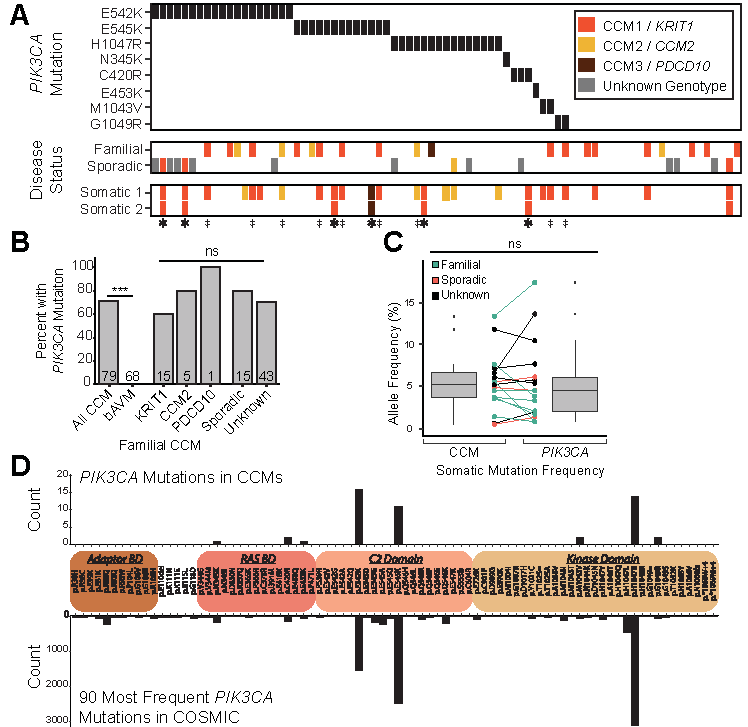
\includegraphics[width=5in]{PIK_discovery}
\end{center}
\caption[Familial and Sporadic CCM Harbor Somatic Mutations in \italicize{PIK3CA}.] {\textbf{Somatic activating \italicize{PIK3CA} mutations are detected in CCMs.} \\ \textbf{A},  A schematic summary of the germline and somatic mutations in \italicize{KRIT1}, \italicize{CCM2} and \italicize{PDCD10}, and the somatic mutations in \italicize{PIK3CA}. Color denotes the affected CCM gene. Samples listed as neither familial nor sporadic are deidentified banked CCMs lacking either clinical information or genetic evidence supporting either classification. * indicates familial CCMs with an activating mutation in \italicize{PIK3CA} and both germline and somatic mutations in a CCM gene. \ddag  ~ indicates known or presumed sporadic CCMs with an activating mutation in \italicize{PIK3CA} and two somatic mutations in a CCM gene. \textbf{B}, Distribution of activating mutations in \italicize{PIK3CA} present in sporadic CCMs, all three forms of familial CCMs, and control brain AVMs.  \textbf{C}, The relationship between somatic \italicize{PIK3CA} and CCM mutations and \italicize{PIK3CA} activating mutations is graphed. Points indicate individual mutations in either a CCM gene or \italicize{PIK3CA}. Lines connect the CCM gene and PIK3CA gene mutations present in a single sample. \textbf{D}, The distributions of somatic \italicize{PIK3CA} mutations identified in human CCMs (top) and cancer (bottom) as reported in COSMIC. ns indicates P not significant; P$>$0.05. *** indicates P$<$1$^{-16}$}

\label{PIK_discovery}
\end{figure}
%%%%%%%%%%%%%%%%%%%%%%%%%%%%%%

\subsection{CCMs Harbor Multiple Somatic Mutations in Different Genes}
Previous studies have demonstrated that human CCM lesions harbor somatic mutations in one of the three causal CCM genes. In this cohort, somatic mutations in CCM genes were identified in 24/79 (30\%) of CCM lesions. The relatively low discovery rate of somatic CCM mutations may reflect types of mutations that are not detectable with short-read sequencing, such as large indels or chromosomal rearrangements. Notably, in the CCM lesions in which we positively identified a somatic loss of function CCM mutation, 21/24 (88\%) also harbored a somatic gain of function \italicize{PIK3CA} mutation. This apparent enrichment in the co-detection of CCM and \italicize{PIK3CA} somatic mutations is consistent with poor sample quality that reduced sensitivity and/or low variant allele frequency in many lesions. Thus the true frequency of \italicize{PIK3CA} mutations in CCM lesions is likely to be higher than the 71\% reported above. The identification of multiple mutations in CCM genes is consistent with the previously described two-hit model of CCM pathogenesis with the addition of a third hit in \italicize{PIK3CA}.  In 9 samples of familial CCM (\ddag ~ on Figure~\ref{PIK_discovery}A), we detected distinct loss of function germline and somatic mutations in the same CCM gene in addition to a gain of function mutation in \italicize{PIK3CA} for a total of 3 genetic hits. In 6 samples of presumed sporadic CCM (*  on Figure~\ref{PIK_discovery}A), we detected two distinct loss of function somatic mutations in the same CCM gene in addition to a gain of function mutation in \italicize{PIK3CA} for a total of 3 genetic hits. These data indicate that no fewer than three independent somatic mutation events contributed to the pathogenesis of those lesions. A comparison of variant allele frequency between CCM and \italicize{PIK3CA} somatic mutations in lesions where both mutations were found revealed no significant correlation (P $>$ 0.15) (Figure~\ref{PIK_discovery}C). This balanced mutation frequency is consistent with a pathogenic mechanism in which both CCM and \italicize{PIK3CA} somatic mutations arise in a single cell during lesion formation, or one in which CCM mutant cells and \italicize{PIK3CA} mutant cells co-exist in similar numbers. Finally, the specific mutant \italicize{PIK3CA} alleles identified in resected human CCM lesions closely mirrored those identified in human cancers in the COSMIC database (Figure~\ref{PIK_discovery}D), consistent with a shared molecular and cellular mechanism. 

\subsection{\italicize{PIK3CA} and CCM/\italicize{MAP3K3} Mutations in the Same Cell}
The identification of both \italicize{PIK3CA} and CCM gene somatic mutations in CCMs raises a critical question: Do these mutations occur in the same cell, or are these mutations in two distinct clonal populations that intermix to form a CCM. To address this question we performed single-nucleus DNA sequencing (snDNA-seq) on 3 sporadic and 2 familial CCMs using the Tapestri platform \citep{xu2019}. Nuclei isolated from frozen tissue were stained with DAPI and subjected to fluorescence-activated nucleus sorting to isolate single nuclei for input into the Tapestri instrument, where the nuclei were partitioned into droplets and the exons of \italicize{KRIT1}, \italicize{CCM2}, \italicize{PDCD10}, and \italicize{PIK3CA} were amplified (Figure~\ref{PIK_singlecell}A). Bulk sequencing of sample 5003 identified one somatic mutation in \italicize{PIK3CA} and two somatic mutations in \italicize{KRIT1}. These same somatic mutations were identified in the snDNA-seq data which show that the majority of somatic mutant nuclei harbored all three mutations. In sporadic CCMs 5038 and 5079 only one somatic CCM gene mutation was called in addition to the \italicize{PIK3CA} somatic mutation. In sample 5079 the second somatic CCM gene mutation is clearly present in total reads, however due to poor efficiency of the amplicon there were insufficient reads per nuclei to reliably establish cellular phase with the other two mutations. Data from both 5038 and 5079 show that the majority of mutant cells harbor both the somatic \italicize{PIK3CA} and CCM gene mutations. Likewise snDNA-seq data for familial CCMs 5065 and 5073 show the majority of somatic mutant nuclei (excluding nuclei with only the germline CCM gene mutation) harbor the \italicize{PIK3CA} mutation and both CCM gene mutations (Figure~\ref{PIK_singlecell}B). While the majority of somatic mutant nuclei in all 5 samples harbor all of the identified somatic mutations, notably there is a smaller number of nuclei observed with each possible combination of genotypes. This observation is highly unlikely to reflect genuine biology as the creation of all genotypes would require identical somatic mutations to occur in multiple clonal populations within the CCM. Some of the observed genotype combinations may represent intermediate clonal populations that formed prior to acquiring the full set of mutations, however the majority of these genotype combinations are likely due to allelic dropout (ADO)---a common technical artifact in single-nucleus/cell DNA sequencing data and has been noted by many previous studies \citep{xu2019, szulwach2015, satas2018}. To estimate the rate of ADO for each sample we identified heterozygous SNPs called in the snDNA-seq data and evaluated the ratio of heterozygous to homozygous nuclei and determined the rate of ADO to be 8.4\% $\pm$ 4.1\%. We also observed dropout of the constitutional CCM pathogenic allele as evidenced by the presence of WT nuclei in familial CCM samples 5065 and 5073. As a result of ADO, the number of nuclei with all somatic mutations is likely underestimated in each sample. Despite the confounding effects of ADO, all 5 samples clearly indicate that the \italicize{PIK3CA} and CCM gene somatic mutations occur in the same cell.

%%%%%%%%%%%%%%%%%%%%%%%%%%%%%%
%				     FIGURE 2					%
%%%%%%%%%%%%%%%%%%%%%%%%%%%%%%
\begin{figure}[tbp!]
\begin{center}
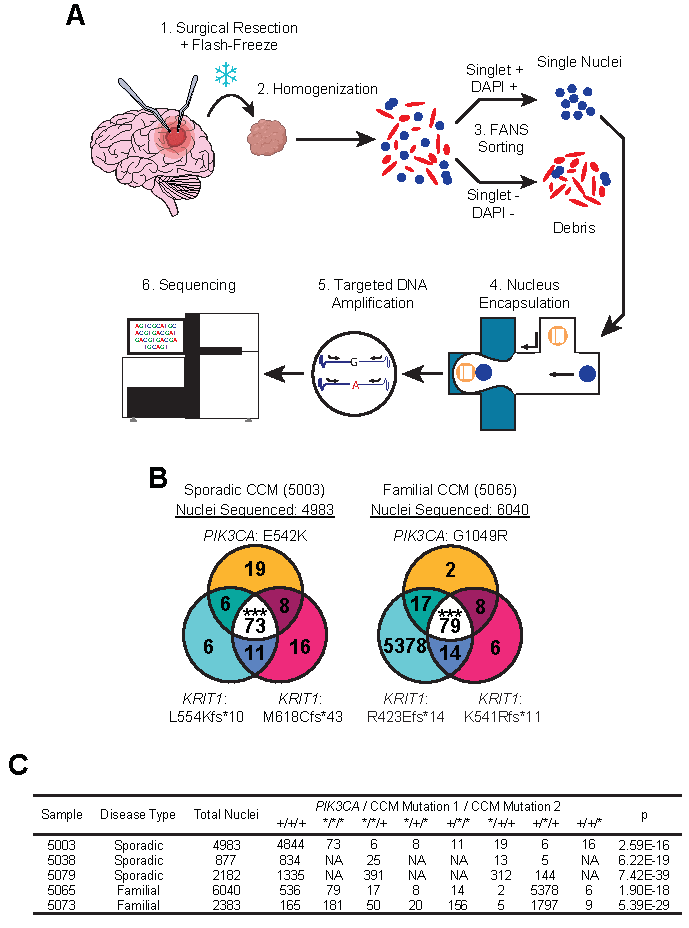
\includegraphics[width=4.5in]{PIK_singlecell}
\end{center}
\caption[Single-Nucleus Sequencing of CCMs with Three Pathogenic Mutations.] {\textbf{Single-Nucleus Sequencing of CCMs with Multiple Mutations.} \\ \textbf{A}, Schematic of workflow for processing frozen surgically-resected human CCM lesions for single-nucleus DNA sequencing. \textbf{B}, Representative data for sporadic and familial CCMs detailing the number of nuclei with each combination of \italicize{PIK3CA} and CCM mutations. *** indicates P$<$1$^{-16}$. \textbf{C}, A summary of snDNA-seq results for 3 sporadic and 2 familial CCMs analyzed is shown. The number of nuclei with each possible genotype are listed. + indicates a wild-type allele; * indicates a mutant allele. Note that only 1 somatic CCM mutation was identified in samples 5038 and 5079. P values were determined by $\chi$-squared test between the observed and expected triple mutant nuclei (or double mutant for lesions 5038 and 5079) determined by Poisson distribution (see Methods).}

\label{PIK_singlecell}
\end{figure}
%%%%%%%%%%%%%%%%%%%%%%%%%%%%%%

\section{Discussion}
These studies demonstrate powerful synergy between mutations that confer loss of CCM function and gain of \italicize{PIK3CA} function in both mouse models of CCM disease and a majority of resected human CCMs. These findings provide new insight into the mechanisms underlying the puzzling natural history of this vascular disease, explain why the disease has not been successfully modeled in mature mice with CCM loss of function alone, and reveal a compound genetic disease mechanism for vascular malformation that is highly analogous to that elucidated for human cancer. Translationally, they also provide strong evidence that approved drugs capable of inhibiting the downstream PI3K effector mTOR, and perhaps the PI3K pathway generally, may be used to block the growth and neurologic complications of clinically symptomatic CCM lesions.  

\subsection{Three-Hit Model of CCM Pathogenesis}
The most significant conceptual advance of this study is the discovery of a compound genetic mechanism of vascular malformation pathogenesis. To date, vascular malformations have been considered monogenic in origin, due either to bi-allelic loss of function mutations (e.g HHT \citep{snellings2019}, CM-AVM \citep{lapinski2018}, previously CCM \citep{akers2009, mcdonald2014}, or mono-allelic gain of function mutations (e.g. Sturge-Weber syndrome \citep{shirley2013}, sporadic bAVM \citep{nikolaev2018}, venous malformations \citep{limaye2015}, lymphatic malformations \citep{luks2015}, and blue rubber bleb nevus \citep{soblet2017, tang2017, goss2019, davis2020, francis2019, couto2017, couto2015}. Our studies identify a digenic, “triple-hit” mechanism involving the acquisition of as many as three distinct genetic mutations that culminate in loss of CCM gene function and gain of \italicize{PIK3CA} function as the basis for rapidly growing, clinically symptomatic CCMs. Thus, aggressive CCM lesions arise via the acquisition of multiple somatic mutations that synergize in a manner similar to that of established cancer drivers. By analogy to cancer, the CCM genes may be considered vascular “suppressor genes”, required to constrain vessel growth, while \italicize{PIK3CA} may be considered a vascular “oncogene”, capable of driving excess vascular growth. As in cancer, the combined loss of a vascular suppressor and gain of a vascular activator is a potent combination that culminates in aggressive, symptomatic disease. Significantly, the present study demonstrates that either CCM loss of function or \italicize{PIK3CA} gain of function alone are sufficient to confer a modest vascular phenotype. These less aggressive vascular lesions are analogous to benign tumors that become malignant after mutation of another driver gene, a scenario consistent with clinical reports of sudden aggressive growth in small, pre-existing CCM lesions. Whether distinct synergistic driver gene combinations underlie other vascular malformations is an important future question that may be addressed by deeper genomic sequencing of human vascular malformations. 

\subsection{Role of Clonal Expansion in Mutagenesis}
A key question raised by our studies is how CCM loss of function and \italicize{PIK3CA} gain of function interact at the cellular and molecular levels during lesion genesis. Insights gleaned from both genetic analysis of human CCM lesions and mouse genetic models are highly complementary and support an endothelial cell autonomous mechanism in which the two pathways are both directly and indirectly linked. Single cell genomic DNA sequencing of both sporadic and familial human CCM lesions reveals that a majority of mutant cells harbor acquired mutations in both a CCM gene and \italicize{PIK3CA}, strong evidence of interaction at the single cell level and that the majority of clonal expansion occurs after acquisition of all three mutations. Aileen Ren showed that sporadic lesions arise in \italicize{Slco1c1}(BAC)-CreERT2;\italicize{Krit1}$^{fl/fl}$;R26-LSL-\italicize{Pik3ca}$^{H1047R}$ animals due to Cre leak that is exclusively endothelial, identifying the endothelial cell as the target cell type and, like the human genetic sequencing data, suggestive of a clonal mechanism in which emergence of a single compound mutant endothelial cell is sufficient for lesion formation.

\subsection{Therapeutic Implications}
Our identification of \italicize{PIK3CA} activation in CCM immediately suggests that PI3K inhibitors may be an effective therapeutic for CCM. \italicize{PIK3CA} mutations are extremely common in cancers. As a result, there is decades of extensive research on the mechanism of \italicize{PIK3CA} activation and many efforts to develop cancer therapies targeting this signaling axis. Among these therapeutics is rapamycin---an off-patent small-molecule drug targeting mTOR (a downstream effector of \italicize{PIK3CA})---which may be made cheaply available to CCM patients. To test the efficacy of rapamycin for preventing CCM, Aileen Ren developed a mouse model with both biallelic CCM loss of function, and \italicize{Pik3ca} gain of function. These mice develop aggressive lesions soon after induction. Aileen showed that rapamycin is extremely effective in preventing lesion formation in these mice \citep{ren2021}. This preliminary data suggests that rapamycin may be a good candidate for pre-clinical trials, though the true test will be whether rapamycin is able to regress existing lesions. Lesion prevention is of course a step forward but given the non-trivial side effects of rapamycin, it is unlikely that long-term treatment will be a viable option. In contrast, if rapamycin is able to regress lesions, then a treatment program may consist of brief intermittent periods of dosing which would more amenable to the patient population. 

\subsection{DVA Predispose to CCM and Other PI3K-Related Diseases}
A clinical clue to the pathogenesis of human CCM disease that may be explained by our findings is the observation that sporadic CCMs frequently arise at sites of pre-existing developmental venous anomalies (DVAs) (24--32\% assessed by MRI, and up to 100\% in one study that assessed this relationship at the time of surgical resection \citep{wurm2005, porter1999, abdulrauf1999}). Since DVAs are benign and do not undergo surgical resection, there are no data addressing their genetic basis.  However, DVA is found in a majority of individuals with Cowden’s syndrome, an inherited disease caused by germline heterozygous loss of function mutations in \italicize{PTEN} that is also the result of PI3K gain of function \citep{dhamija2018, tan2007}.  A parsimonious explanation for these clinical observations is that endothelial cells with pre-existing \italicize{PIK3CA} mutations sufficient to confer DVA subsequently acquire CCM loss of function mutations and transform into more aggressive sporadic CCM lesions.  While such a clinical pathogenesis remains entirely speculative until DVA genetic sequencing is performed, it would support a mechanism highly analogous to cancer in which accrued mutations convert a benign vascular abnormality into a more malignant one. 

\section{Methods}
\subsubsection{CCM Collection}
Human CCM tissue specimens were obtained from surgically resected specimens from three sources including the Barrow Neurological Institute, Angioma Alliance biobank, and University of Chicago. This study was approved by each institutions respective Institutional Review Board. 

\subsubsection{Brain AVM Collection}
Brain AVM tissue specimens were obtained from the nidal tissue of surgically resected brain AVMs (M.T.L). For non-vascular lesion controls (NVLCs), temporal lobe specimens were similarly acquired from subjects undergoing anterior temporal lobectomies for medically refractory epilepsy. All tissues were frozen at -80$^{\circ}$C and stored in a biobank. This study was approved by the University of California San Francisco Institutional Review Board and performed in compliance with the Health Insurance Portability and Accountability Act regulations.

\subsubsection{DNA Extraction}
DNA from human CCM samples was extracted using the DNeasy Blood and Tissue Kit (Qiagen). Extractions were done as per the manufacturers’ directions excepting cases where less than 25mg of tissue was available. For samples $<$25mg the manufacturer recommended volumes were either halved or quartered---depending on the amount of tissue available---to optimize final DNA concentration and yield. Final DNA concentrations were quantified using Qubit dsDNA BR assay kit (Invitrogen cat. Q32850) according to manufacturer recommended protocol. 

\subsubsection{Droplet Digital PCR}
Identification of somatic \italicize{PIK3CA} mutations was performed using droplet digital PCR (ddPCR) according to manufacturer protocol for mutation detection assays (BioRad 10047489 Ver B). For each sample with sufficient DNA yield, 30--100ng of DNA was incorporated into droplets using the QX200 AutoDG system (BioRad). After PCR, fluorescence from the resulting droplets was read using the QX200 droplet reader (BioRad). These steps were repeated for three assays testing the presence of the three most common \italicize{PIK3CA} mutations: E542K, E545K, and H1047 (ThermoFisher assay IDs: Hs000000085\_rm, Hs000000086\_rm, Hs000000088\_rm, respectively). Each assay included a no-template control, a wild-type control, and a mutation-positive control for the mutation being assayed. The mutation-positive controls were DNA extracted from cell lines with known heterozygous mutation of E542K (T84), E545K (HCT15), or H1047R (HCT116).  The output of the droplet reader was analyzed using the QuantaSoft software (BioRad). The gates for positive and negative mutation status were drawn with respect to the distribution of droplets in the mutation-positive controls and applied to all samples. 

\subsubsection{SNaPshot}
Human CCM samples with an E542K, E545K, or H1047R \italicize{PIK3CA} mutation identified by sequencing or ddPCR underwent tertiary confirmation of mutation status using SNaPshot (Applied Biosystems), a single-base extension sanger sequencing assay. An initial round of PCR amplified exons 9 and 20. In a second round of PCR, primers directly adjacent to the assayed nucleotide was extended with ddNTPs and sequenced on a 3130 Genetic Analyzer (Applied Biosystems). Sequences were examined using GeneMapper software (Applied Biosystems). The allele frequency of the mutation by dividing the area under the peak of the mutant allele by the total area under both allele peaks. The primers used in this analysis were synthesized according to designs in a previously published assay for \italicize{PIK3CA} mutations \citep{hurst2009}.

\subsubsection{Sequencing}
Previous studies identifying somatic mutations in CCMs and bAVMs have reported alternate allele frequencies less than 1\%. To enable the detection of variants at such low frequencies we aimed to sequence samples to an average of 1000x (actual mean coverage 1102x) coverage in addition to leveraging 10bp unique molecular identifiers (UMIs) to mitigate the impact of PCR duplication. These conditions allow us to theoretically detect variants as low as 0.5\% allele frequency. 

Sequencing libraries for the human CCMs and bAVMs were prepared using the SureSelect XT HS target enrichment workflow (Agilent). The targeting panel used for sequencing the CCMs covers the following genes: \italicize{KRIT1}, \italicize{CCM2}, \italicize{PDCD10}, \italicize{PIK3CA}, \italicize{PTEN}, \italicize{AKT1} ,\italicize{KRAS}, \italicize{RAF}, \italicize{NRAS},\italicize{MAP2K1}, \italicize{RASA1}, \italicize{TEK}, \italicize{GNAQ}, \italicize{GNA11}, \italicize{MAP2K2}, \italicize{PPP2R5D}, \italicize{ACVRL1}, \italicize{ENG}, \italicize{SMAD4}, \italicize{AKT2}, \italicize{AKT3}, \italicize{CCBE1}, \italicize{CDKN1C}, \italicize{FLT1}, \italicize{FLT4}, \italicize{FOXC2}, \italicize{GATA2}, \italicize{GDF2}, \italicize{GJC2}, \italicize{GLMN}, \italicize{KIF11}, \italicize{MTOR}, \italicize{PIK3R2}, \italicize{PTPN14}, \italicize{SOX18}, \italicize{STAMBP}, \italicize{VEGFC}, \italicize{MAP2K4}, \italicize{MAP3K1}, \italicize{MAPK1}, \italicize{JAK1}, \italicize{JAK2}, \italicize{JAK3}, \italicize{KDR}, \italicize{NOTCH1}, \italicize{PDGFRA}, \italicize{PDGFRB}, \italicize{RET}, \italicize{HRAS}, \italicize{TP53}, \italicize{MSH2}, \italicize{MYB}, \italicize{MYCN}, \italicize{MYC}, \italicize{ERBB2}, \italicize{EGFR}, \italicize{NTRK2}, \italicize{ODC1}, \italicize{SLC25A21}, \italicize{PTTG1}, \italicize{TSC1}, \italicize{TSC2}, \italicize{EPHB2}, \italicize{TGFBR1}, \italicize{TGFBR2}, \italicize{TGFBR3}. 

The bAVM samples were sequenced using a customized Agilent Comprehensive Cancer panel which covers 175 genes including \italicize{PIK3CA}. After library preparation, CCM samples were pooled and sequenced across 1 lane of a HiSeq4000 (illumina) with paired-end 150bp reads. bAVM samples were pooled and sequenced across a NovaSeq6000 SP flow cell (illumina) with paired-end 150bp reads. 

\subsubsection{Sequence Analysis}
Sequencing data was processed according to the GATK (Broad Institute) best practices for somatic short variant discovery with slight modifications for “tumor-only” sequencing data. As a secondary method for variant discovery we developed custom software designed specifically for the detection of somatic mutations in sequencing data from samples with no available normal tissue. This software was implemented as part of Gonomics, an ongoing effort to develop an open-source genomics platform in the Go programming language. Gonomics can be accessed at github.com/vertgenlab/gonomics. 

After variant calling the resulting variants were functionally using snpEff. In this process each variant was annotated with: the protein-level consequence of coding mutations: the predicted impact of missense mutations according to SIFT, PolyPhen2, and PROVEAN; membership in several SNP databases including dbSNP, 1000 Genomes project, and ExAC; and membership in the Catalogue of Somatic Mutations in Cancer (COSMIC). We filtered the resulting list of variants using the following inclusion criteria: $>$100x total coverage; $>$5 supporting reads; $<$90\% strand specificity; $>$0.5\% alternate allele frequency; $<$1\% population allele frequency according to the above mentioned SNP databases; and membership in the COSMIC database. 

\subsubsection{Single-Nucleus DNA Sequencing}
Frozen human CCM lesion tissue obtained from medically-indicated, surgical resection were prepared for single-nucleus DNA sequencing (snDNA-seq) following a nuclei isolation protocol by Martelotto L. (dx.doi.org/10.17504/protocols.io.3fkgjkw). All steps prior to loading on the Tapestri platform were performed in $<$3 hours. Nuclei were maintained at 4$^{\circ}$C throughout the protocol. Frozen tissue was homogenized by Dounce in Nuclei EZ Lysis Buffer (Sigma-Aldrich), briefly washed, filtered through a 70$\mu$m mesh, stained with DAPI, and filtered through a 35$\mu$m mesh. The CCM homogenate was sorted using a FACSAriaII (BD) (70$\mu$m nozzle, 70psi, 4-Way Purity, chiller) gating to retain singlet DAPI-positive events (Figure~\ref{PIK_supplement}). Up to 400,000 sorted nuclei were collected in 1ml of the following buffer prepared with ultrapure nuclease-free water: Na$_2$SO$_4$ 82mM, K$_2$SO$_4$ 30mM, glucose 10mM, HEPES 10mM, MgCl$_2$ $\cdot$ 6H2O 5mM, BSA 2\%. Sorted nuclei were pelleted by centrifugation at 4$^{\circ}$C (500rcf, 10min), supernatant discarded, and resuspended in 36$\mu$L of MissionBio Cell Buffer. The concentration of nuclei was determined by counting DAPI-positive nuclei with a hemocytometer on an EVOS FL (fluorescence) microscope (Thermo Fisher) while confirming that nuclei aggregates comprised $<$5\% of total nuclei. Samples with $<$5\% aggregate nuclei and a concentration within 2000--4000 nuclei/$\mu$L (diluting with additional MissionBio Cell Buffer where necessary) were used for snDNA-seq.

%%%%%%%%%%%%%%%%%%%%%%%%%%%%%%
%				     FIGURE 3					%
%%%%%%%%%%%%%%%%%%%%%%%%%%%%%%
\begin{figure}[tbp!]
\begin{center}
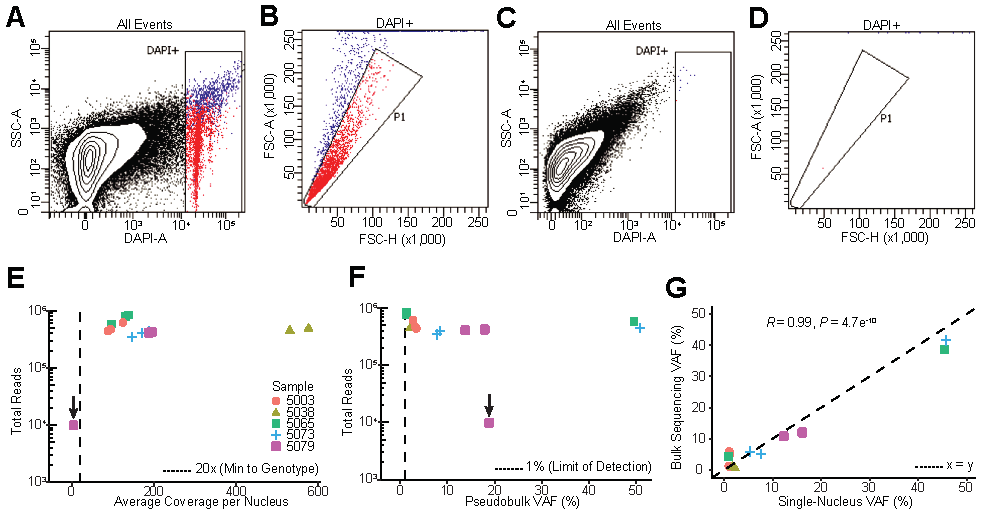
\includegraphics[width=6in]{PIK_supplement}
\end{center}
\caption[Correspondence of Bulk and Single-Nucleus Sequencing.] {\textbf{Correspondence of Bulk and Single-Nucleus Sequencing.} \\ \textbf{A-D}, Representative FANS plots of DAPI stained (A-B) and unstained (C-D) CCM homogenate samples. Doublet discrimination by forward scatter profile for DAPI stained and unstained samples are shown in B and D respectively. \textbf{E}, Total reads and average coverage per nucleus from snDNAseq for each mutation detected by bulk sequencing. Dotted line shows 20x coverage, the minimum cutoff used for establishing genotype.  \textbf{F}, Pseudobulk allele frequency from snDNA-seq for each mutation detected by bulk sequencing. Dotted line shows 1\% allele frequency. Note the data point with * in E-F shows a mutation in sample 5079 detected in bulk sequencing which, due to poor amplification during snDNA-seq, received insufficient coverage per nucleus (4.5x) to establish nuclear genotypes however is clearly present in pseudobulk reads (1849/9814). \textbf{G}, Comparison of mutation allele frequency as detected by bulk and snDNA-seq. As nuclei are diploid for the relevant autosomes, the x-axis is equal to the fraction of mutant nuclei divided by two. Dotted line shows perfect correlation at x=y. \italicize{R} and \italicize{P} were calculated by Pearson’s correlation coefficient. }

\label{PIK_supplement}
\end{figure}
%%%%%%%%%%%%%%%%%%%%%%%%%%%%%%

Library preparation was performed using the Tapestri platform (MissionBio) according to the manufacturers protocol (PN3354). Libraries were generated with a custom amplicon panel synthesized by MissionBio covering all exons of \italicize{KRIT1}, \italicize{CCM2}, \italicize{PDCD10}, and 7 amplicons covering somatic mutation hotspots in \italicize{PIK3CA}, per the COSMIC database. Up to three libraries were pooled and sequenced with a NextSeq Mid-Output 2 x 150bp kit (illumina). Data processing and QC was performed by the MissionBio cloud-based analysis pipeline. Data quality for each nuclei barcode was determined using MissionBio recommended filtering settings. Data from low quality nuclei barcodes were removed prior to mutation analysis. 
	
To determine the cellular phase of somatic mutations detected in bulk sequencing, nuclei barcodes were selected that had a minimum of 20x coverage across all mutant regions to ensure that all nuclei included in the analysis have appropriate sensitivity to detect a mutation. For each nuclei barcode and each mutant position, reads containing the ref and alt alleles were counted. Mutant regions that had both a minimum of 10 alt reads and 10\% allele frequency were marked as mutation positive. The number of nuclei barcodes with each possible genotype are recorded in Figure~\ref{PIK_singlecell}C. 
	
The p value for each sample was determined by Chi-squared test comparing the observed number of triple mutant nuclei barcodes (or double mutant if only two mutations were identified) to the expected number of triple mutant nuclei barcodes if the null hypothesis is true. In this test the null hypothesis is that the observed somatic mutations do not occur in the same cell and instead exist in two clonal populations where the proportion of each population = 2 $\cdot$ variant allele frequency (assuming cells are diploid and heterozygous for the mutation). In samples where three somatic mutations were identified an alternative null hypothesis may be to use three clonal populations, however assuming that the three somatic mutations are partitioned into two clonal populations as asserted above is a more conservative test and therefore used here. To determine the expected number of triple mutant nuclei barcodes we first determined the expected number of droplets with two (or more) nuclei by approximating a Poisson distribution. The expected number of triple mutant nuclei barcodes is the product of the number of droplets with two nuclei, the proportion of mutant clone 1, and the proportion of mutant clone 2. 
	
Here we report the Poisson estimation p value as this is the accepted method for estimating the rates of false-positive droplets when dealing with data generated using microfluidics. We can also consider a more intuitive upper bound for the p value by considering the extreme case where each droplet contains two nuclei. In this case the expected number of triple mutant nuclei barcodes is the product of the total number of nuclei barcodes, the proportion of mutant clone 1, and the proportion of mutant clone 2. Even in this extreme case the highest p value among our data is $<$1 $\times$ $10^{-17}$. 

\section{Contributions and Acknowledgements}
This chapter is adapted from a study published in \italicize{Nature} (Ren \& Snellings et al., 2021) with the following authors:  Aileen A. Ren, Daniel A. Snellings, Sophie Y. Su, Courtney C. Hong, Marco Castro, Alan T. Tang, Matthew R. Detter, Nicholas Hobson, Romuald Girard, Sharbel Romanos, Rhonda Lightle, Thomas Moore, Robert Shenkar, Christian Benavides, M. Makenzie Beaman, Helge Mueller-Fielitz,  Mei Chen, Patricia Mericko, Jisheng Yang, Derek C. Sung, Michael T. Lawton, Michael Ruppert, Markus Schwaninger, Jakob K\"{o}rbelin, Michael Potente, Issam A. Awad, Douglas A. Marchuk and Mark L. Kahn. AAR and DAS contributed equally to this study. AAR designed and performed most of the mouse and tissue culture experiments and wrote the manuscript. DAS performed the genetic studies of human CCM lesions and wrote the manuscript. SYS created and performed the adult cranial window assays in mice. CCH, ATT and MRD contributed to mouse genetic studies. MC performed in vitro studies. NH, RG, SR, RL, TM, RS and IAA performed microCT CCM lesion imaging and quantification in a blinded manner. MC and PM assisted with mouse genetic studies. JY and DCS performed histologic studies. MTL provided surgically excised human CCM samples. MS and JK provided critical reagents. MP, IAA, DAM and MK designed experiments and wrote the manuscript.

We thank the members of the Kahn lab for their thoughtful comments and advice during this work. We thank Angioma Alliance for patient enrollment, and the University of Chicago PaleoCT core facility for its expertise in imaging and image quantitation. We thank the Penn CDB Microscopy Core for support with microscopy. Flow cytometry was performed in the Duke Human Vaccine Institute Research Flow Cytometry Shared Resource Facility. We thank Duke University School of Medicine for use of the Sequencing and Genomic Technologies Shared Resource for library preparation and sequencing. These studies were supported by National Institute of Health grants R01HL094326 and R01NS100949 (MK), P01NS092521 (MK, DM, IA) the Leducq Foundation (MK, MP), the AHA-Allen foundation (MK), T32 HL007150 (AR), F31HL152738 (DS), F31NS115256 (CH), F30NS100252 (AT), European Research Council (ERC) Synergy Grant-2019-WATCH-810331 (MS) and ERC Consolidator Grant EMERGE-773047 (MP).

